\chapter{Implementation and Results}

This chapter focuses on comparing the performance between \acrshort{mcmc} and \acrshort{vi} methods for performing inference in a \acrshort{pgm}. Each method have their strengths and weaknesses for different types of problems. As a compromise, this chapter will focus on comparing the performance of a fictitious model in order to discuss a concrete example.  

\section{The model}
As the context of this paper is intention inference for autonomous ferries, it seems fit that a similar example is used. A simple intention model is therefore proposed as an example, which relates steering angle to an intention through a mixture model. 

The angle $\theta_t$ is defined to be the angle between the obstacles current course and the predicted course given the obstacles final destination. If the obstacles reported final destination is correct, $D_t=0$, the angle should be closely related to the obstacles intention and can be generated from a Gaussian selected by the intention $I_t$ (i.e. a mixture of Gaussians weighted by the intention probabilities). If the obstacle report an incorrect destination, $D=1$, the angle $\theta_t$ is independent of intention.

This example model is intentionally not identifiable only from observing the angles $\theta_t$. However, through the use of informative priors, the model is still able to learn from data. 

Whether or not the final destination is valid is modelled using a Bernoulli variable $D_t$ which takes the value $1$ if the destinations is \textbf{invalid}. A Beta distribution is used to model the prior probability of $D=1$, i.e. the destination being invalid.  

\begin{equation}
    p_D \sim \text{Beta}, \quad p_D \in (0, 1)
\end{equation}
\begin{equation}
    D_t \sim \text{Bernoulli}(p_D), \quad D_t \in \{0, 1\}
\end{equation}

The intention in a situation $I_t$ is modelled by a Categorical discrete variable where the possible realizations are shown in \cref{tbl:intentions}. The intention probabilities $\boldsymbol{\alpha}$ are distributed according to a Dirichlet distribution.

\begin{equation}
    \boldsymbol{\alpha} \sim \text{Dirichlet}, \quad \boldsymbol{\alpha} \in \{\alpha_0, \alpha_1, \alpha_2 \in (0, 1) \; | \; \sum_i \alpha_i = 1 \}
\end{equation}
\begin{equation}
    I_t \sim \text{Categorical}(\boldsymbol{\alpha}), \quad I_t \in \{0, 1, 2\}
\end{equation}

\begin{table}[h]
\centering
\begin{tabular}{|l|l|}
\hline
$I_t=0$ & The obstacle intends to keep its current course \\ \hline
$I_t=1$ & The obstacle intends a starboard turn           \\ \hline
$I_t=2$ & The obstacle intends a portside turn            \\ \hline
\end{tabular}
\caption{Possible realizations of the intention $I_t$}
\label{tbl:intentions}
\end{table}


The mixture components for $\theta_t$ when $D_t=0$ are Gaussian Distributions. For $I=0$, the mean is zero with unknown variance. For $I \in \{1, 2\}$ the means have equal absolute value, but opposite sign. The absolute value for $\mu_2 = -\mu_1$ and the variance $\sigma^2$ are unknown. The variance is assumed equal for all intentions. 
Learning the mean $\mu_2 = -\mu_1$ from data allows the model to adapt to different types of ships. A small fishing vessel might rapidly change course (i.e. large $\theta_t$), while a large oil-tanker has limited ability to turn due to its size (i.e. smaller $\theta_t$). 
\begin{align}
    \mu_0 &= 0 &  \mu_{1} = - \mu_{2} &\sim \text{Gaussian} & \sigma &\sim \text{Inv-Gamma}
\end{align}
When $D=0$ and $I_t=i$, the angle is distributed according to
\begin{equation}\label{eq:theta_intention_mixture}
    p(\theta_t | D=0, I_t=i) = \mathcal{N}(\mu_i, \sigma^2), \quad \theta_t \in \mathcal{R}
\end{equation}

The distribution of $\theta_t$ when $D_t=0$ becomes the Gaussian mixture model in \cref{eq:angle_gauss_mixture}.

\begin{align}\label{eq:angle_gauss_mixture}
\begin{split}
    p(\theta_t | \boldsymbol{\mu}, \sigma, D=0) = &\Pr\{I_t=0\}\mathcal{N}(\theta_t | \mu_0, \sigma^2)\\
    &+ \Pr\{I_t=1\}\mathcal{N}(\theta_t | \mu_1, \sigma^2)\\
    &+ \Pr\{I_t=2\}\mathcal{N}(\theta_t | \mu_2, \sigma^2)
\end{split}
\end{align}

One issue with using a Guassian distribution for angle information is that it has support on $\mathcal{R}$, while the angles $\theta$ should ideally only have support on $(-\pi, \pi)$. In practice, this may not be a big issue as long as the probability mass is mostly kept within $(-\pi, \pi)$. Another solution could be to use a nonlinear transformation to clamp $\mathcal{R}$ to $(-\pi, \pi)$.

\cref{fig:intention_angle} shows the likelihood for different angles for the different intentions with fixed mean and variance. 

When the obstacles target destination is invalid, $D=1$, the angle $\theta$ is distributed according to a Uniform distribution over the range $(-\pi, \pi)$ to model how the angle contains no information about the obstacle in such a case. 

\begin{equation}\label{eq:angle_uniform}
    p(\theta_t | D=1) = \text{Uniform}(-\pi, \pi)
\end{equation}

The distribution for $\theta_t$ becomes a mixture between the Gaussian Mixture in \cref{eq:angle_gauss_mixture} and the uniform distribution in  \cref{eq:angle_uniform} as expressed in \cref{eq:angle_complete_mixture} by the law of total probability.

\begin{align}\label{eq:angle_complete_mixture}
\begin{split}
     p(\theta_t | \boldsymbol{\mu}, \sigma)
     &= \sum_D \Pr\{D=d\} p(\theta_t | D=d, \boldsymbol{\mu}, \sigma)\\
     &= \Pr\{D_t = 0\} \underbrace{p(\theta_t | \boldsymbol{\mu}, \sigma, D_t=0)}_{\text{\cref{eq:angle_gauss_mixture}}} + \Pr\{D_t=1\}\underbrace{p(\theta_t | D_t=1)}_{\text{\cref{eq:angle_uniform}}}
\end{split}
\end{align}


The data generating process for $\theta_t$ then becomes:

\begin{enumerate}
    \item Draw priors $p_D$, $\boldsymbol{\alpha}$ 
    \item Draw priors $\mu_i$ and $\sigma_i$ for all intentions 
    \item Draw $D_t$ and $I_t$ conditional on $p_D$ and $\boldsymbol{\alpha}$
    \item If $D_t=1$, draw $\theta_t$ from Uniform distribution. If not, draw $\theta_t$ from $\mathcal{N}_{I=i}$ conditional on $\mu_i$ and $\sigma_i$.
\end{enumerate}


The resulting joint distribution can then be factored into \cref{eq:example_joint}.

\begin{align}\label{eq:example_joint}
\begin{split}
    &p(\theta_t, I_t=i, D_t=d, \boldsymbol{\mu}, \sigma, p_D, \boldsymbol{\alpha})\\
    &= \underbrace{p(\theta_t | I_t=i, D_t=d, \boldsymbol{\mu}, \sigma)}_{\text{\cref{eq:angle_complete_mixture}}}\underbrace{p(I_t=i | \boldsymbol{\alpha})}_{\text{Categorical}}\underbrace{p(D_t=d)}_{\text{Bernoulli}}\underbrace{p(\boldsymbol{\alpha})}_{\text{Dirichlet}}\underbrace{p(p_D)}_{\text{Beta}}\underbrace{p(\boldsymbol{\mu})}_{\mathcal{N}} \underbrace{p(\sigma)}_{\text{Inv-Gamma}}
\end{split}
\end{align}


\begin{figure}
    \centering
    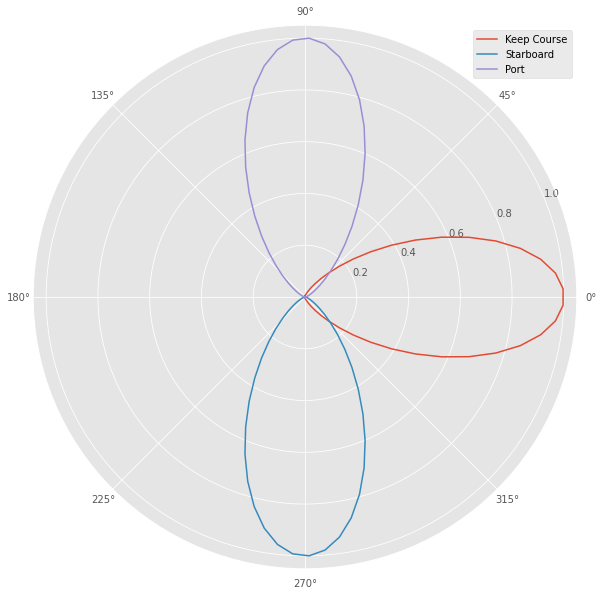
\includegraphics[width=0.7\textwidth]{figures/intention_angle.png}
    \caption{Normalized likelihood of different angles under different intention hypotheses. This is a polar plot where the angle represent $\theta_t^{(I=i)}$, the radius represent the probability. This is generated from \cref{eq:theta_intention_mixture} with $\mu_0=0$, $\mu_1 = -\frac{\pi}{2}$, $\mu_2=\frac{\pi}{2}$ and $\sigma_i=\frac{\pi}{8}$}
    \label{fig:intention_angle}
\end{figure}

\subsection{Priors}
The priors are shown in \cref{fig:priors}.
\begin{figure}
    \centering
    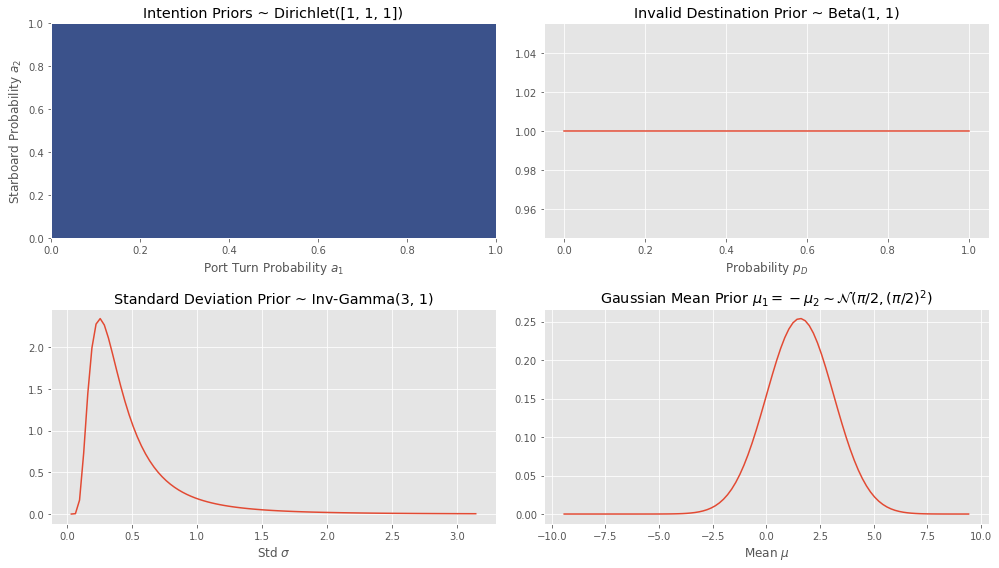
\includegraphics[width=1\textwidth]{figures/priors.png}
    \caption{Model priors for $\boldsymbol{\alpha}$, $p_D$, $\sigma$ and $\boldsymbol{\mu}$. The contour plot for $\boldsymbol{\alpha}$ shows $\alpha_1$ and $\alpha_2$, but $\alpha_0$ is implicitly included by the constraint $\alpha_0 = 1 - \alpha_1 - \alpha_2$. The priors for $\boldsymbol{\alpha}$ and $p_D$ are non-informative priors, while the priors for $\mu_2 = -\mu_1$ and $\sigma$ are informative priors selected by intuitive reasoning.}
    \label{fig:priors}
\end{figure}

\section{Implementation}
Both \acrshort{mcmc} and \acrshort{vi} were implemented using Tensorflow Probability, as it has great support for both methods as well as it utilizes Tensorflows automatic differentiation to avoid dealing with error-prone calculations \cite{tensorflow2015-whitepaper}. The joint distribution in \cref{eq:example_joint} was implemented using the \texttt{JointDistributionSequential} distribution in TFP. (TODO: Add code in appendix)


\section{Dataset \& Benchmark}
The dataset was generated from $N=100$ samples $\boldsymbol{\mathcal{D}}$ from \cref{eq:angle_complete_mixture} with fixed parameters. The amount of samples was intentionally kept low, as the need for Bayesian methods usually arise when the amount of data is sparse. A successful inference should be able to regain the parameters $\boldsymbol{\alpha}$, $p_D$, $\mu_2 = -\mu_1$ and $\sigma$ from $\mathcal{D}$.

\section{Markov Chain Monte Carlo}
Hamiltonian Monte Carlo was implemented using Tensorflow Probability (TFP). The log posterior target density was specified as 
\begin{align}\label{eq:example_ll}
\begin{split}
    ll &= \sum_{t=1}^N \log p(I_t, D_t, \boldsymbol{\mu}, \sigma, p_D, \boldsymbol{\alpha} | \theta_t = \mathcal{D}_t)\\
    &\propto \sum_{t=1}^{N}\log p(\theta_t = \mathcal{D}_t, I_t, D_t, \boldsymbol{\mu}, \sigma, p_D, \boldsymbol{\alpha})
\end{split}
\end{align}

The proposal distribution were transformed using the following transformations (Bijectors)

\begin{itemize}
\item SoftmaxCentered was used to achieve unconstrained sampling for $\boldsymbol{\alpha} \in (0, 1)^3$.
\item Sigmoid was used to achieve unconstrained sampling for $p_D \in (0, 1)$
\item Softplus was used to achieve unconstrained sampling for $\sigma > 0$
\end{itemize}

$100$ chains were randomly initialized using samples from the prior and then sampled independently in parallel. Each chain consists of $2500$ samples, where the first $500$ samples are discarded due to burn-in. This results in $2000 \cdot 100 = 200000$ samples in total. 

\section{Variational Inference}

\acrshort{vi} was implemented using a transformed Gaussian mean-field approximation. Each variable is approximated using an independent, transformed Gaussian distribution as surrogate density. Specifying this model was easily achieved by passing a list of Bijectors to \texttt{tfp.experimental.vi.build\_factored\_surrogate\_posterior}. 

The Stochastic Gradient Descent (SGD) optimizer \texttt{tf.optimizers.Adam} was then used to optimize the KL divergence by passing it to \texttt{tfp.vi.fit\_surrogate\_posterior} along with the same log posterior density used for \acrshort{mcmc}, expressed in \cref{eq:example_ll} \cite{tensorflow2015-whitepaper}. 

\section{Results}

\subsection{Observation One: More data yields better results}
Two datasets were randomly generated using the same fixed parameters in \cref{tbl:example_case_1_params}, but with different number of samples. The first dataset consists of $N_1=500$ samples, while the second contains twice as many with $N_2=1000$ samples. 

The
\begin{table}[h]
\centering
\begin{tabular}{lllll}
\textbf{Variable:}   & $\boldsymbol{\alpha}$ & $p_D$ & $\boldsymbol{\mu}$                  & $\sigma$         \\ \hline
\textbf{True value:} & $[0.7, 0.3, 0.1]$     & $0.3$ & $[0, -\frac{\pi}{2}, \frac{\pi}{2}]$ & $\frac{\pi}{16}$
\end{tabular}
\caption{True values used to generate the dataset for example case 1.}
\label{tbl:example_case_1_params}
\end{table}

\begin{figure}[h]
    \centering
    \begin{subfigure}{\textwidth}
    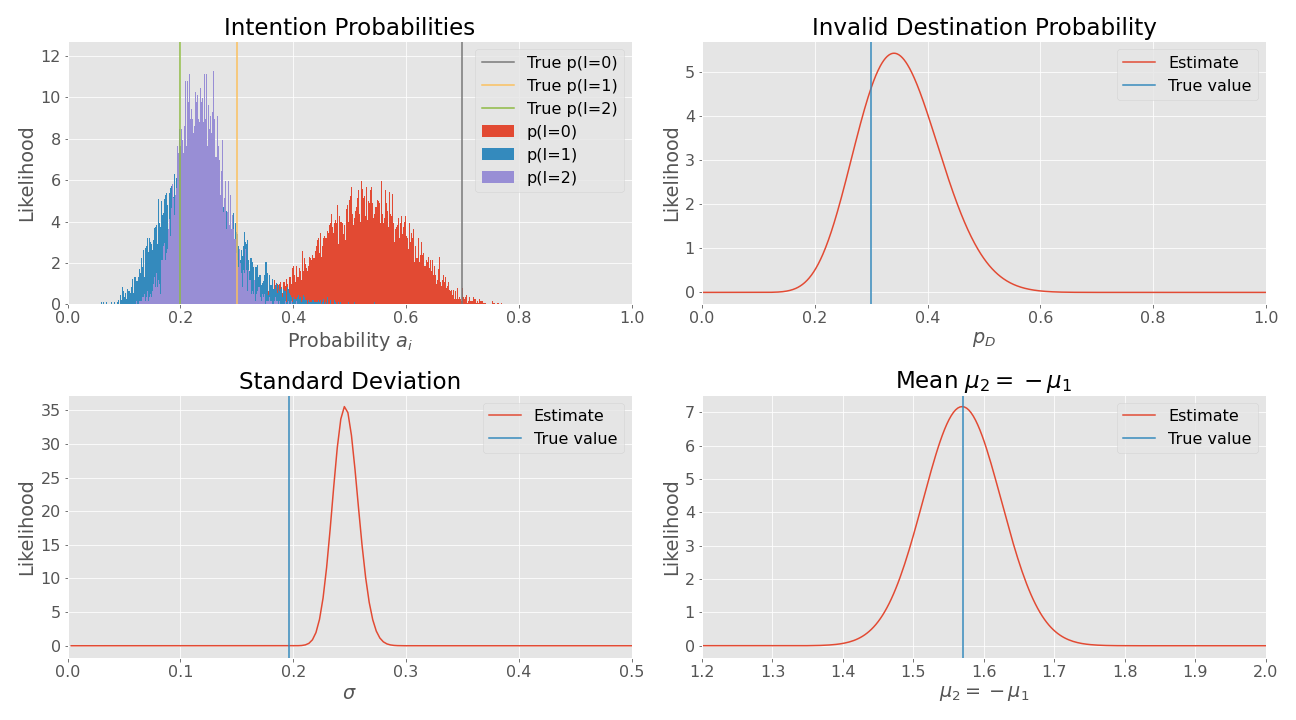
\includegraphics[width=\textwidth]{figures/example_1_vi_posterior.png}
    \caption{\acrshort{vi}}
    \end{subfigure}
    \begin{subfigure}{\textwidth}
    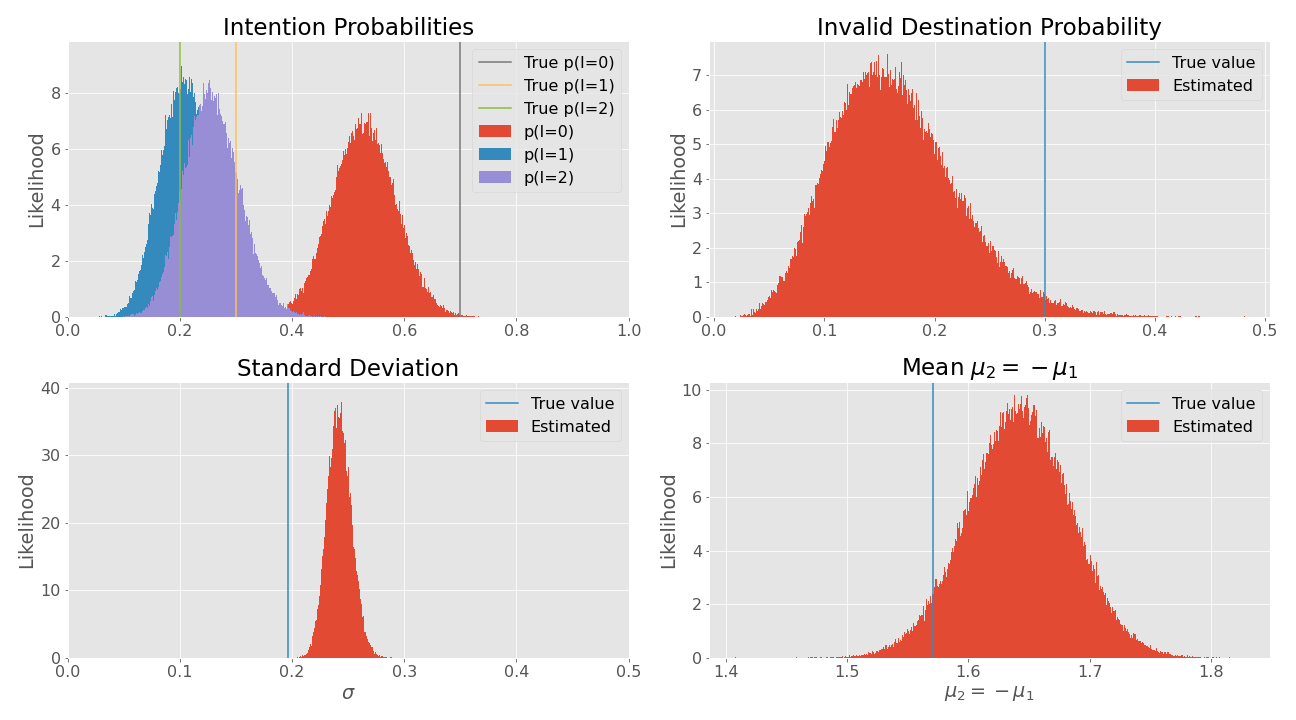
\includegraphics[width=\textwidth]{figures/example_1_mcmc_posterior.png}
    \caption{\acrshort{mcmc}}
    \end{subfigure}
    \caption{Posterior Distribution for example case 1 using \acrshort{vi} and \acrshort{mcmc} methods for inference}
    \label{fig:example_case_1_vi}
\end{figure}